\newpage
\section{White Rabbit PTP Core}

The WR PTP (Precision Time Protocol) Core (WRPC) \cite{WR-core:wiki} \cite{WR-core:manual} \cite{WRPC:ohwr}, figure \ref{fig:WRPC}, is an Ethernet MAC implementation capable of providing precise timing. 
It can be used for sending and receiving regular Ethernet frames between user-defined HDL modules and a physical medium. 
It also implements the White Rabbit protocol to provide sub-nanosecond time synchronization.

\vspace{5 mm}

\noindent The White Rabbit PTP Core can operate in one of the following modes:
 
\begin{itemize}
\item GrandMaster:
    \begin{itemize}
    \item[>] WR Master synchronized to an external 1-PPS and 10 MHz clock signal, propagates precise timing to other WR-compliant devices.
    \end{itemize}
\item Master:
    \begin{itemize}
    \item[>] WR Master with free-running oscillator, propagates precise timing to other WR-compliant devices.
    \end{itemize}
\item Slave:
    \begin{itemize}
    \item[>] synchronizes its internal oscillator to another WR Master device.
    \end{itemize}
\end{itemize}

\begin{figure}[H]
    \centering
    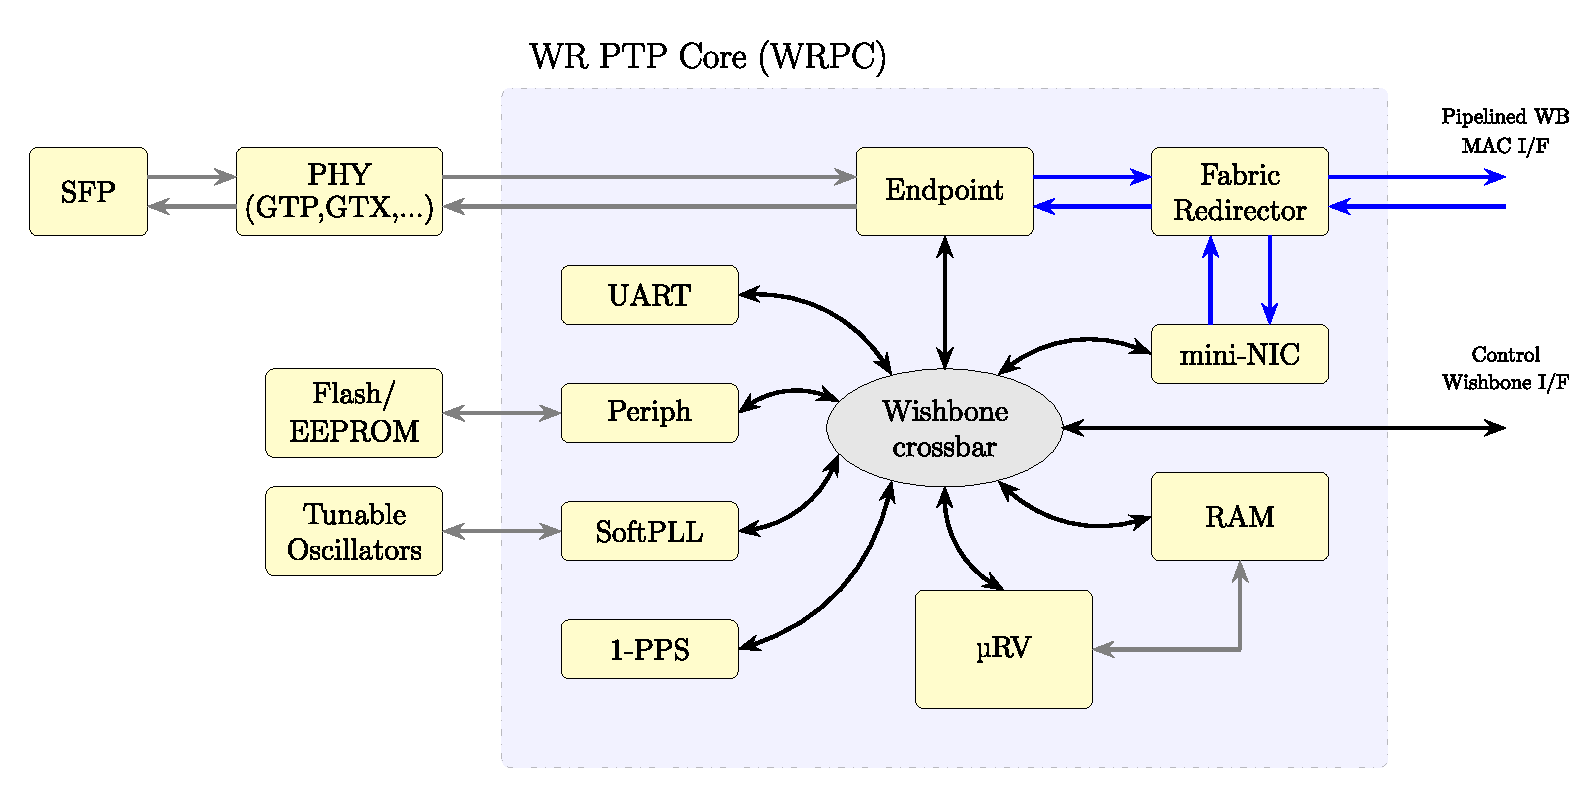
\includegraphics[width=15cm]{figures/WRPC.pdf}
    \caption{WR PTP (Precision Time Protocol) Core (WRPC).}
    \label{fig:WRPC}
\end{figure}

\noindent You can find the HDL description of the WRPC internal components in \cite{WRPC:modules}.

\subsection{\textmu RV}

The \textmu RV \cite{urv-core:ohwr} \cite{urv-core:wiki} \cite{Włostowski:2213516} (Micro RISC-V) core is a small-sized implementation of a 32-bit RISC-V core, targeted specifically at FPGAs developed by CERN. 

\begin{figure}[H]
    \centering
    
\includegraphics[width=5cm]{figures/urv_logo.png}
    \caption{\textmu RV logo.}
    \label{fig:urv}
\end{figure}

\begin{itemize}
\item Features:
    \begin{itemize}
    \item[>] Supports RV32IM instruction set. 
Division and multiply high instructions are optional and can be emulated to lower the FPGA footprint.
    \item[>] Target: FPGAs.
    \item[>] 4-stage pipeline (FDXW).
    \item[>] All instructions except taken branches/division in one clock cycle.
    \item[>] Code execution from internal memory block.
    \item[>] Wishbone bus (version B.4) for peripheral access.
    \item[>] Simple interrupt handling.
    \item[>] Verilog RTL code.
    \end{itemize}
\end{itemize}

\noindent Since \textmu RV is described in verilog and most of the WRPC component is in VHDL, it will be necessary to use a \textbf{mixed simulator} supported by VUnit.
In this context, one of the best options is \say{QuestaSim}.

\vspace{5mm}

\noindent \href{https://github.com/umarcor}{Umarcor} is planning to develop a container, hosted on our server, for this purpose. 
(DONE - Questa container, with and without VUnit, available on the lab server.)

\vspace{5mm}

\noindent \textbf{Task:} Learn how to generate a testbench using both HDLs: VHDL and Verilog.
(Initial mixed simulation test DONE - Unfortunately questa is a proprietary software and our server image cannot be distributed, so this example cannot be shown on GitHub, it is only available in our private GitLab repository.)

\subsection{WRPC Simulation}

I've successfully simulated WRPC \cite{WRPC:ohwr} in its \say{v4.2} version for \textbf{Spartan6} FPGA.

\vspace{5mm}

\noindent See \href{https://github.com/Unike267/Thesis/issues/2}{github.com/Unike267/Thesis/issues/2} to check how I have done it.

\vspace{5mm}

\noindent HDL modules that form the WRPC (\say{v4.2} for Spartan6) are:

\newpage 

\begin{dig}
\item ip\_cores
    \begin{dig}
    \item etherbone-core
        \begin{dig}
        \item hdl
            \begin{dig}
            \item eb\_master\_core (VHDL)
            \item eb\_slave\_core (VHDL)
            \item eb\_usb\_core (VHDL)
            \end{dig}
        \end{dig}
    \item general-cores
        \begin{dig}
        \item modules
            \begin{dig}
            \item common (VHDL)
            \item genrams
                \begin{dig}
                \item . (VHDL)
                \item common (VHDL)
                \item generic (VHDL)
                \item xilinx (VHDL)
                \end{dig}
            \item wishbone
                \begin{dig}
                \item . (VHDL)
                \item wb\_async\_bridge (VHDL)
                \item wb\_axi4lite\_bridge (VHDL)
                \item wb\_bus\_fanout (VHDL)
                \item wb\_clock\_crossing (VHDL)
                \item wb\_crossbar (VHDL)
                \item wb\_dma (VHDL)
                \item wb\_dpram (VHDL)
                \item wb\_gpio\_port (VHDL)
                \item wb\_i2c\_bridge (VHDL)
                \item wb\_i2c\_master (VHDL)
                \item wb\_irq (VHDL)
                \item wb\_lm32
                    \begin{dig}
                    \item generated (Verilog and VHDL)
                    \item platform/spartan6 (Verilog)
                    \item src (Verilog and VHDL)
                    \end{dig}
                \item wb\_onewire\_master (Verilog and VHDL)
                \item wb\_serial\_lcd (VHDL)
                \item wb\_simple\_pwm (VHDL)
                \item wb\_simple\_timer (VHDL)
                \item wb\_slave\_adapter (VHDL)
                \item wb\_spi (Verilog and VHDL)
                \item wb\_spi\_flash (VHDL)
                \item wb\_uart (VHDL)
                \item wb\_vic (VHDL)
                \item wbgen2 (VHDL)
                \item wbgenplus (VHDL)
                \end{dig}
            \end{dig}
        \item platform/xilinx
            \begin{dig}
            \item wb\_xil\_multiboot (VHDL)
            \item wb\_xilinx\_fpga\_loader (VHDL)
            \end{dig}
        \end{dig}
    \item gn4124-core
        \begin{dig}
        \item hdl
        \begin{dig}
            \item gn4124core   
                \begin{dig}
                \item rtl
                    \begin{dig}
                    \item . (VHDL)
                    \item spartan6 (VHDL)
                    \end{dig}  
                \end{dig}            
            \item spec
                \begin{dig}
                \item ip\_cores (VHDL)
                \end{dig}  
            \end{dig}
        \end{dig}
    \end{dig}
\item modules
    \begin{dig}
    \item fabric
        \begin{dig}
        \item . (VHDL)
        \item xwrf\_loopback (VHDL)
        \end{dig}
    \item timing (VHDL)
    \item wr\_dacs (VHDL)
    \item wr\_eca (VHDL)
    \item wr\_endpoint (VHDL)
    \item wr\_mini\_nic (VHDL)
    \item wr\_pps\_gen (VHDL)
    \item wr\_si57x\_interface (VHDL)
    \item wr\_softpll\_ng (VHDL)
    \item wr\_streamers (VHDL)
    \item wr\_tbi\_phy (VHDL)
    \item wr\_tlu (VHDL)
    \item wrc\_core (VHDL)
    \end{dig}
\item platform
    \begin{dig}
    \item xilinx
        \begin{dig}
        \item . (VHDL)
        \item wr\_gtp\_phy
            \begin{dig}
            \item . (VHDL)
            \item spartan6 (VHDL)
            \end{dig}
        \end{dig}
    \end{dig}
\end{dig}

\newpage 

\noindent HDL files for simulation are:

\begin{dig}
\item sim
    \begin{dig}
    \item endpoint\_mdio.v
    \item endpoint\_regs.v
    \item eth\_packet.svh
    \item if\_wb\_link.svh
    \item if\_wb\_master.svh
    \item if\_wb\_slave.svh
    \item if\_wishbone\_accessor.svh
    \item if\_wishbone\_types.svh
    \item lbk\_regs.v
    \item minic\_regs.vh
    \item simdrv\_defs.svh
    \item tbi\_utils.sv
    \item wb\_fabric\_defs.svh
    \item wb\_packet\_sink.svh
    \item wb\_packet\_source.svh
    \item wrc\_syscon\_regs.vh
    \item drivers:
        \begin{dig}
        \item simdrv\_minic.svh
        \item simdrv\_wr\_endpoint.svh 
        \end{dig}
    \end{dig}
\item testbench
    \begin{dig}
    \item wrc\_core
        \begin{dig}
        \item main.sv 
        \item functions.svh 
        \end{dig}
    \end{dig}
\end{dig}
